\begin{table}[h]
  \footnotesize
  \centering
  \begin{tabular}{c c c c}
    \toprule
    Application & Knobs & Utility & Dataset \\
    \midrule
    \specialcell{Pedestrian\\Detection}
                & \specialcell{resolution \\ frame rate \\ quantizer }
                & F1 score & \specialcell{training: MOT16-04\\testing: MOT16-03} \\
    \midrule
    \specialcell{Augmented\\Reality}
                & \specialcell{resolution \\ frame rate \\ quantizer }
                & F1 score & \specialcell{iPhone video clips\\training: office (24 s)\\testing: home
    (246 s)} \\
    \midrule
    \specialcell{Top-k}
                & \specialcell{head (N) \\ threshold (T) }
                & \specialcell{Kendall's $\tau$}
                        & \specialcell{sec.gov access log~\cite{edgarlog} \\ training: 4 days \\
    testing: 16 days} \\
    \bottomrule
  \end{tabular}
  \caption{\sysname{} Applications}
  \label{tab:apps}
\end{table}

\section{Implementation}
\label{sec:implementation}

In this section we present details about our implementation, including a
prototype framework and three non-trivial wide-area streaming applications.

\para{Framework:} While our proposed APIs are general and not language specific,
we choose a safe language, Rust, to implement the core framework. \sysname{} is
open-source on Github.\footnote{Url elided for anonymity.} Applications built
with \sysname{} runs as a single process. The entire processing pipeline is
often specified in a single main file. The execution mode (profiling, runtime as
client or runtime as server) is configured with command line arguments or
environment variables. Our deployment manager is currently a shell script.

% First, Rust's memory safety guarantee can ensure applications running
% continously for an extended period of time. Besides, the zero-cost abstraction
% removes the possibilities of tail latencies caused by uncoordinated garbage
% collection~\cite{maas2016taurus}. In addition, we rely on Rust's type system
% to enforce the type match on \texttt{maybe} operations.

% All operators implement the \texttt{Stream} trait which has an associate type
% \texttt{Item} and a core function \texttt{next} that returns
% \texttt{Datum}. Each datum is either an item with the \texttt{Stream::Item} or
% an \texttt{Error} that the operator use to communicate with the runtime
% scheduler. The concrete form of \texttt{maybe} API is almost an direct
% translation of the API specification. While our API specification
% in~\autoref{tab:operators} uses a vector for knobs, our Rust implementation is
% more general: any type (including vector) that implements \texttt{IntoKnob}
% trait can be used as the knob.
% \begin{lstlisting}
% pub trait Stream {
%     type Item;
%     fn next(&mut self) -> Datum<Self::Item, Error>;

%     fn maybe<K, F>(self, opts: K, f: F) -> Maybe<Self, F>
%         where Self: Sized,
%                 K: IntoKnob,
%                 F: FnMut(K::Item, Self::Item) -> Self::Item {

%          // omitted
%     }
% }
% \end{lstlisting}

\para{Applications:} We've built built three applications: pedestrian detection surveillance, an
augmented reality and a distributed log analysis to extract the Top-k most
access filed. \autoref{tab:apps} summarizes the application specific part:
knobs, utility function and the dataset we used for training and testing.

% \begin{figure*}
%   \centering
%   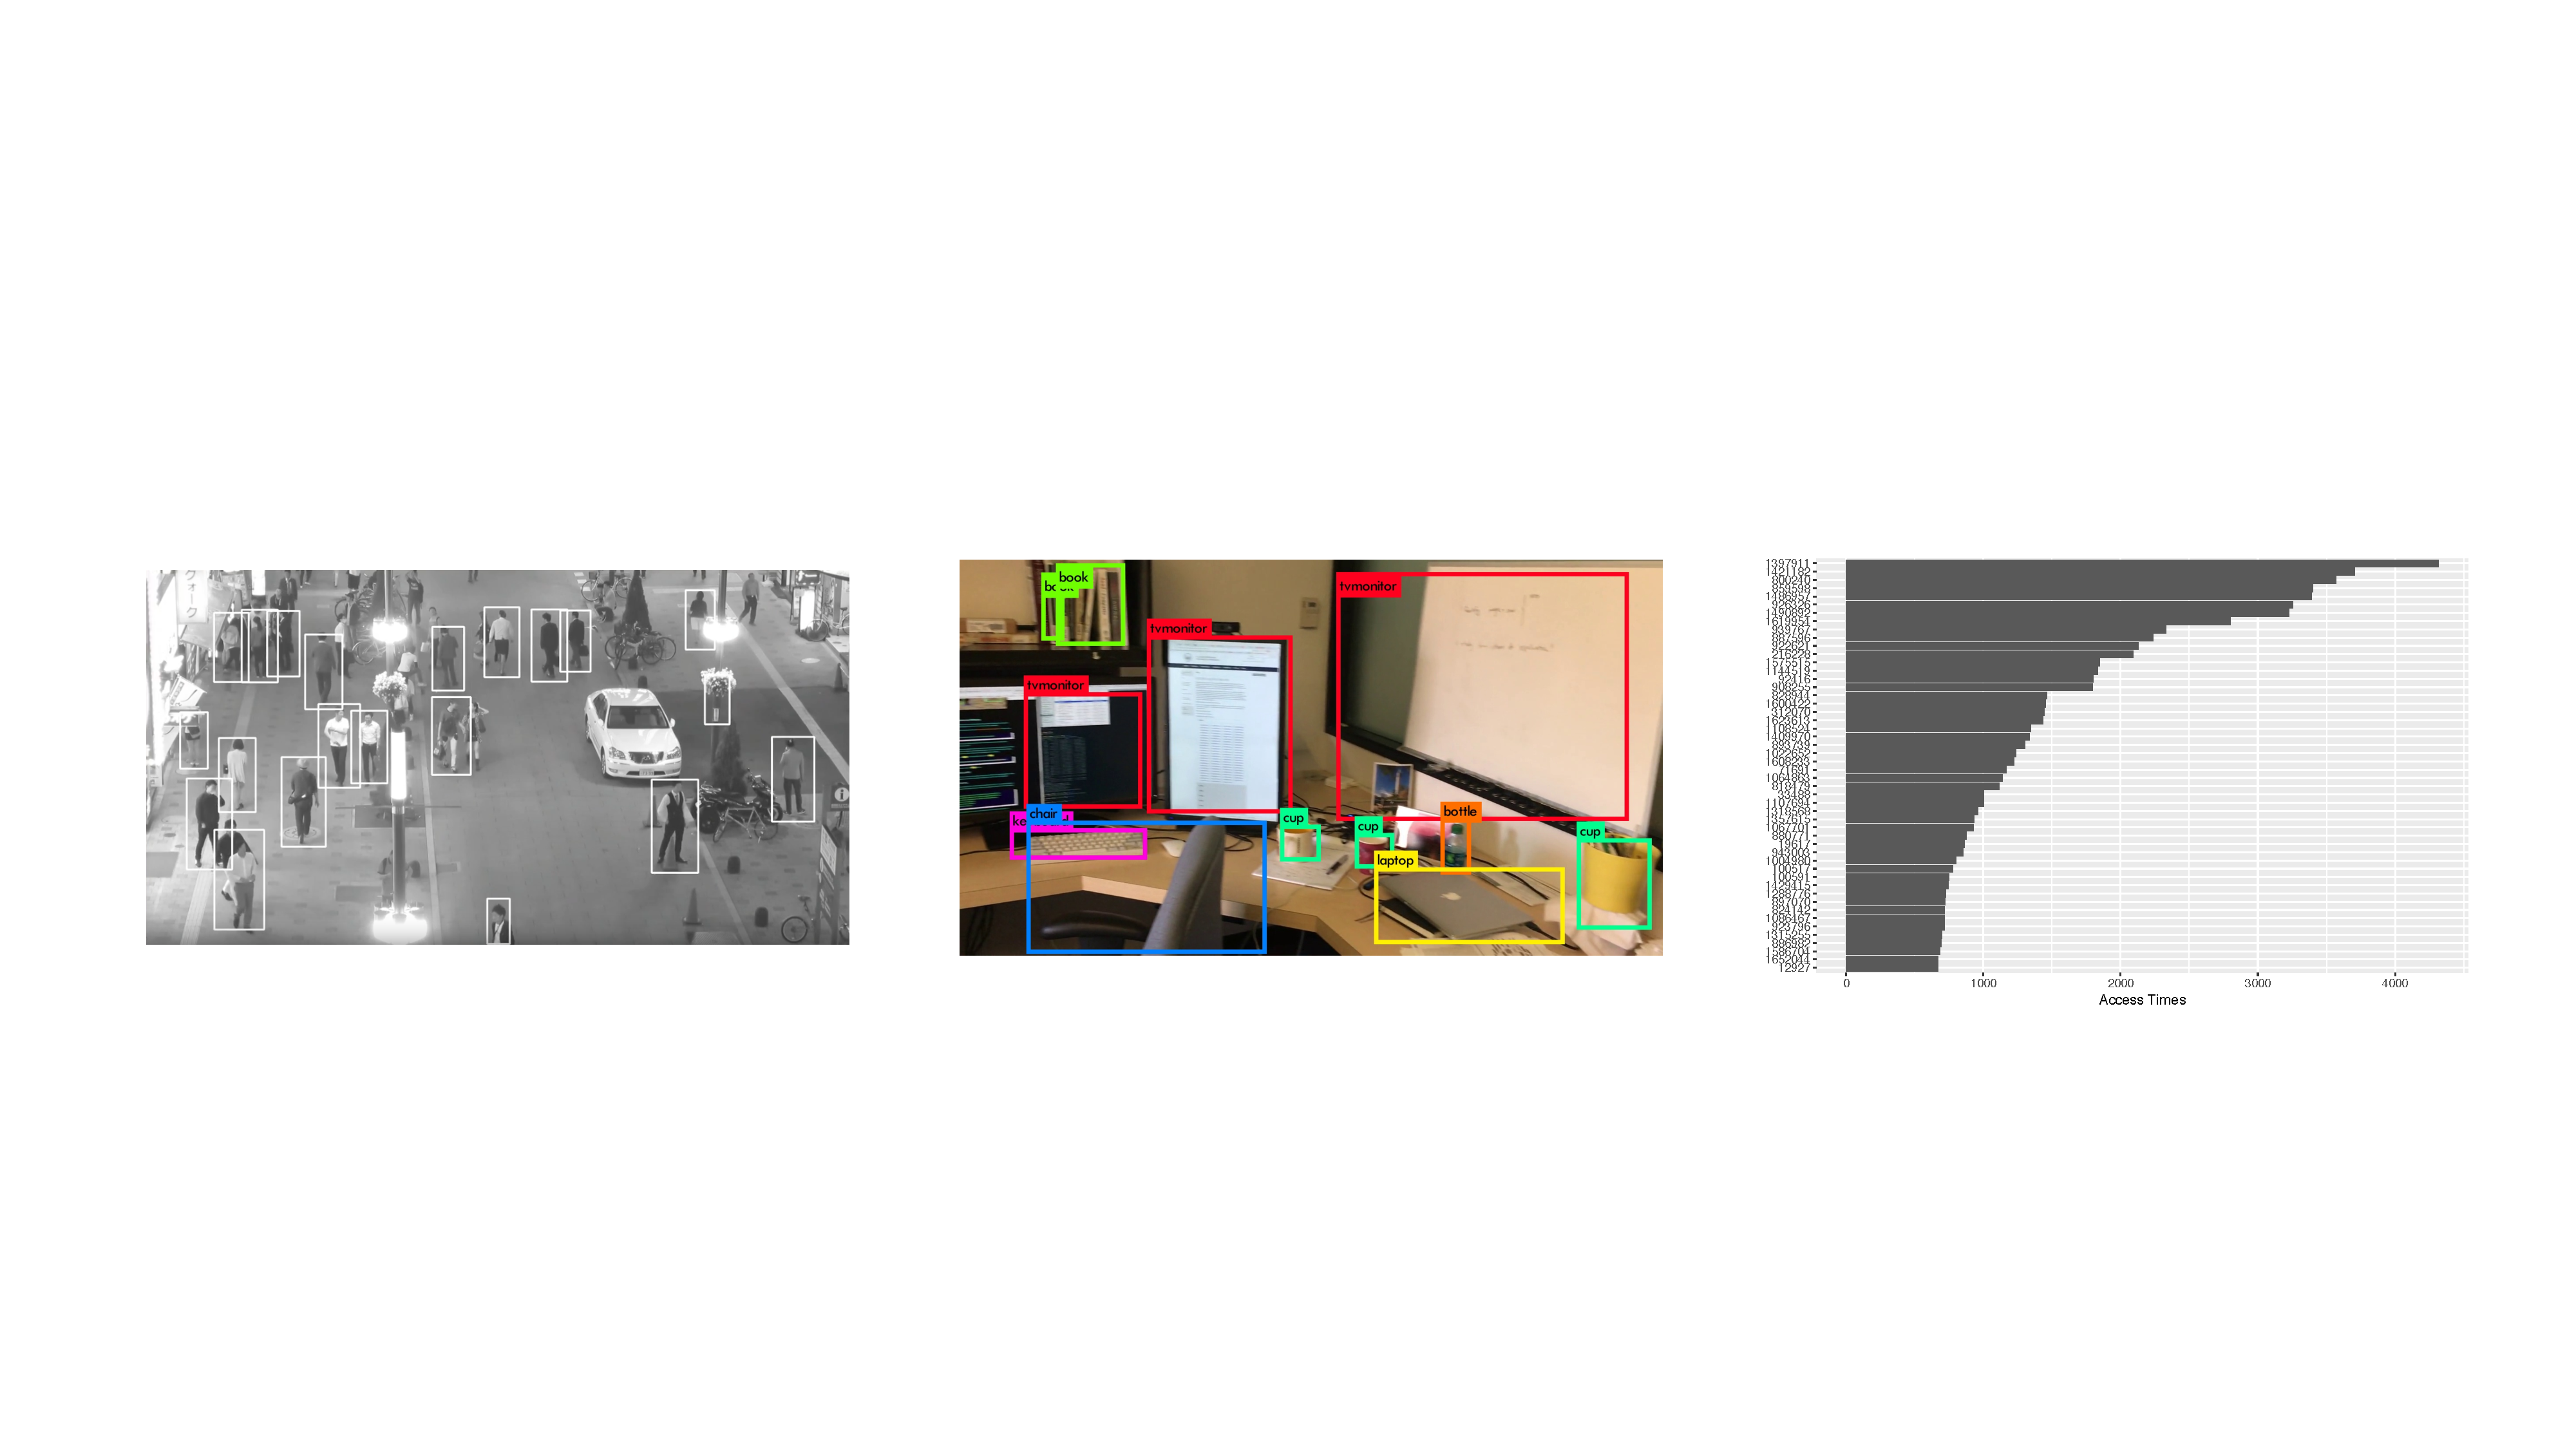
\includegraphics[width=\textwidth]{figures/apps.pdf}
%   \caption{Applications}
%   \label{fig:apps}
% \end{figure*}

\subsection{Building Applications}
\label{sec:build-appl}

\para{Pedestrian Detection:} This application analyzes streams of videos from
installed CCTV cameras and detects pedestrians inside. We implement
image-related operations with OpenCV 3.1~\cite{opencvlibrary}. Pedestrians are
detected using histogram of oriented gradients (HOG)~\cite{dalal2005histograms}
with the default linear SVM classifier. To ensure real-time processing of
frames, we use the GPU-accelerated implementation. Video encoding employs H.264
scheme for its prevalence in existing systems. Our implemenation is based on
GStreamer~\cite{gstreamer} with \texttt{x264enc} plugin. To integrate with
\sysname{}, we first create a pipeline that exposes \texttt{appsrc} (to feed raw
image data) and \texttt{appsink} (to get encoded bytes). The GStreamer main loop
is managed in a separate thread and \sysname{} communicates with it via Rust's
channel. The \texttt{x264enc} is configured with \texttt{zerolatency} present
and uses four threads. Constant quality encoding is used and the quantizer is
exposed as a parameter that can be tuned.

The detection returns a list of bounding boxes, and each box is a rectangle with
normalized coordinates on the image. The detections are compared against the
reference result from raw data. A successful detection is defined when the
intersection over union (IOU) is greater than
50\%~\cite{everingham2010pascal}. For the utility function, we use F1 score
(\%), the harmonic mean of precision and
recall~\cite{Rijsbergen:1979:IR:539927}.

\para{Augmented Reality:} We target at mobile augmented reality applications
that offload the heavy computation to resources elsewhere. Even when the
offloading server is nearby~\cite{satyanarayanan2009case, zhang2015cloud},
wireless communication link is also susceptible to capacity variation.

We use a similar setup (OpenCV and GStreamer) as the pedestrian detection except
the actual analytical functions. To recognize objects, we use a a pre-trained
neural network~\cite{darknet13, redmon2016yolo9000} with the GPU-accelerated
implementation for real-time processing. Here, a successful detection also
requires matching the object type in addition to the IOU criterion.

\para{Distributed Top-K:} Many monitoring applications need to answer the
``top-k'' question~\cite{babcock2003distributed}, such as the top-k most popular
URLs or the top-k most access files. A distributed top-k application aggregates
informations from geo-distributed servers (see \autoref{fig:topk} for an
illustration).

\begin{figure}
  \centering
  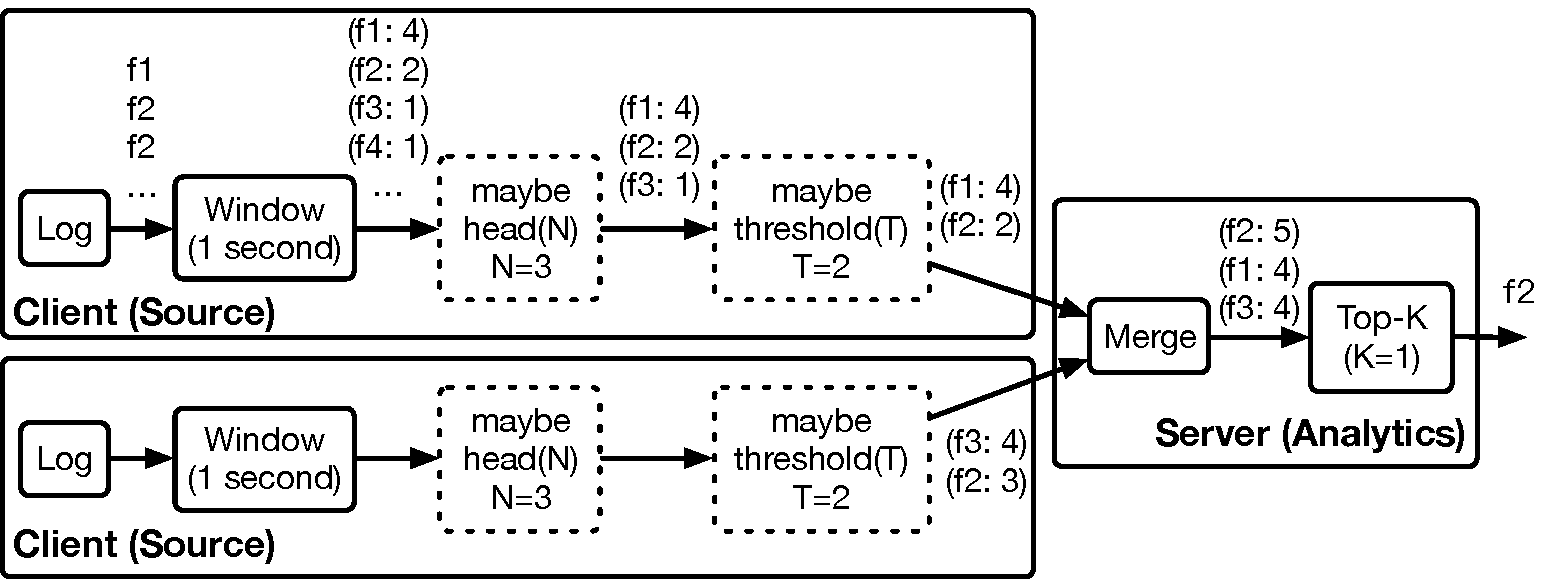
\includegraphics[width=\columnwidth]{figures/topk.pdf}
  \caption{Distributed Top-K Application}
  \label{fig:topk}
\end{figure}

Naively aggregating all the raw logs is not feasible as popular servers have
millions of requests per second. Edge nodes can first perform a \texttt{Window}
operation to generate data summary, such as key-value pairs of \texttt{<item,
  count>}. However, even after this operation, the data size can still be too
large given most real-world access patterns follow a long-tailed
distribution. There is a large-but-irrelevant tail that contributes little to
the final results.

We consider two degradation operations that edge nodes can perform: (1) a head
(\texttt{N}) operation that only takes the top \texttt{N} entries; (2) a
threshold \texttt{T} that filters small entries. These two operations are not
orthognal to each other. Their impact on data size reduction and quality
degradation depends on the distribution of the actual data. For the accuracy, we
use Kendall's $\tau$~\cite{abdi2007kendall}. It is a correlation measure of the
concordance between two ranked list. The output ranges from -1 to 1,
representing no agreement to complete aggrement, respectively. To integrate with
\sysname{}, we convert the measure with a linear transformation to the range of
[0, 1].


\newpage

new column

%%% Local Variables:
%%% mode: latex
%%% TeX-master: "sosp17"
%%% End:
